\section{Heterogeneous Treatment Effects}

\begin{frame}{A Set of Spatial Treatment Effects}
\begin{itemize}
    \item Assume we have finite spatial grid which is divided in $i∗j$ grids, where $i \in Lat$ and $j \in Long$. 
    \vspace{-7pt}
    \item Then, we can obtain a set of treatment effects $D = \{\delta_{1,1}, \delta_{2,1}, \delta_{1,2}, ..., \delta_{i,j}\}$ by subtracting values in their untreated state from the treated state, holding fixed their spatial position at i,j. 
    \vspace{-7pt}
    \item Commonly, it is assumed that all elements of $D$ are constant over space. This assumption does not hold in spatially heterogeneous settings. Those are common in many policy settings, e.g., environmental policy.
\end{itemize}
\end{frame}

\begin{frame}{Reporting Heterogeneous Treatment Effects}

The set of treatment effects $D$ at time $t_i$ may be spatially heterogeneous:  
\vspace{5pt}

  \begin{columns}
    % Split 1
      \begin{column}{0.33\linewidth}
      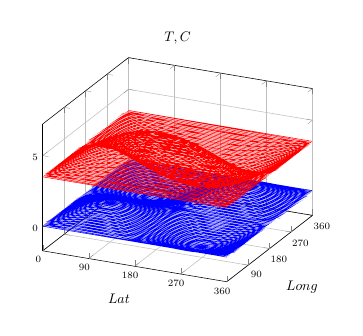
\begin{tikzpicture}[scale=0.50]
      \begin{axis} [
        title = {$T, C$},
        xtick = {0,90,...,360},
        ytick = {90,180,...,360},
        xlabel = $Lat$, ylabel = $Long$,
        ticklabel style = {font = \scriptsize},
	grid]
        \addplot3 [blue, domain=0:360, samples=60] 
        	{ sin(x)*sin(y) };
        \addplot3 [red, domain=0:360, samples=60] 
        	{ sin(0.5*x)*3*sin(y) + 3.5 };
        \end{axis}
        \end{tikzpicture}
        \centering{\footnotesize{Treatment ($T$) and Control ($C$)}}
    \end{column}
    % Split 2
    \begin{column}{0.33\linewidth}
      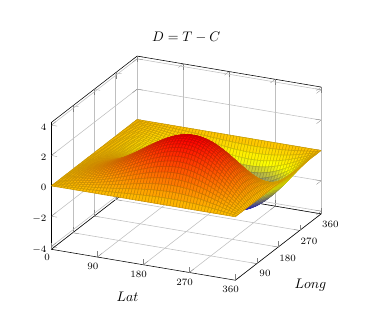
\begin{tikzpicture}[scale=0.50]
      \begin{axis} [
        title = {$D = T - C$},
        xtick = {0,90,...,360},
        ytick = {90,180,...,360},
        xlabel = $Lat$, ylabel = $Long$,
        ticklabel style = {font = \scriptsize},
	grid]
        \addplot3 [surf, domain=0:360, samples=60] 
        	{ sin(0.5*x)*3*sin(y) - sin(x)*sin(y) };
        \end{axis}
        \end{tikzpicture}
        \centering{\footnotesize{Net Treatment Effects ($D$)}}
    \end{column}
    % Split 3
    \begin{tikzpicture}[scale=0.50]
      \begin{axis} [
    title = {$D = T - C$},
    xtick = {0,90,...,360},
    ytick = {90,180,...,360},
    xlabel = $Lat$, ylabel = $Long$,
    ticklabel style = {font = \scriptsize},
    ]
    \addplot3 [contour gnuplot={number=14,labels=false}, domain=0:360, samples=60]
      { sin(0.5*x)*3*sin(y) - sin(x)*sin(y) };
    \end{axis}
    \end{tikzpicture}
  \end{columns}
\end{frame}

\begin{frame}{A Non-parametric Appraoch to Reporting}
- Select k clusters to fit the set of treatment effects
- We go from discrete treatment effects (Dictated by spatial granularity of observations), to continuous interpolation (GPR), then back to discrete treatment clusters (but this time on the basis of heterogeneity clusters). Theoretically, this approach manages to remove bias from structural spatial sampling bias. 
- In the k=1 case we would just report the ATE over all observations
- If there are n units, the k=n case would represent idiosyncratic treatment effects
- Find the best k between 1 and n, 
- k that minimizes the sum of standard errors within the cluster
- Problem: The SSE function is monotonically decreasing and does not have a global minimum
- IMPORTANT CONNECTION: Similar drawback to the overfitting problem - could we borrow tools from the ML repertoire on overfitting?
- It is in a way similar to bias-variance trade-off, aka performance vs. generalizability!!!!!!


- Subtract treatment from control
- Yields another map
- The fact that we subtract smaller subsets of treatment effetcs makes it robust to spatial heterogeneity
- But where is the optimal point of reporting?
\end{frame}

\begin{frame}{Clustering Algorithms}
Pre-defined: Policymakers may choose on a neighborhood (or zip code) basis for instance. However, that could be problematic bc that may permeate existing biases from policymakers. The data may hold information on unobservables that policymakers are unaware of. Instead, I propose a data-driven alternative. 

k-Means:
- Existing solutions: elbow and silhouette method
- Drawback: Only circular shapes

Gaussian Mixture Model algorithm??
- well it is parametric! 

Are there any non-parametric mixture models?

Also we DO NOT want any bias towards density of observations!!!

Also we want to cluster over time subsets, that could be even more difficult and non-intuitive than spatial clusters. The connection of the next-adjacent observation in space AND time is equally important!!

\end{frame}